\documentclass[]{article}

\usepackage{caption,subcaption,graphicx,float,url,amsmath,amssymb,amsthm,tocloft,cancel,thmtools,gensymb,braket,bm}
\usepackage[toc,nonumberlist]{glossaries}
\usepackage{glossaries-extra}
\usepackage[toc,page]{appendix}

\newcommand\numberthis{\addtocounter{equation}{1}\tag{\theequation}}

\newtheorem{thm}{Theorem}
\newtheorem{defn}[thm]{Definition}
\newtheorem{cor}[thm]{Corollary}
\newtheorem{lemma}[thm]{Lemma}
\graphicspath{{figs/}}
\widowpenalty10000
\clubpenalty10000
\setcounter{tocdepth}{2}

%opening
\title{Theoretical Minimum\\Particle Physics 3\\Supersymmetry and Grand Unification}
\author{}

\begin{document}

\maketitle

\begin{abstract}
	These are my notes for the \emph{New Revolutions in Particle Physics 3} lectures from Leonard Susskind's \emph{Theoretical Minimum} series\cite{susskind2010supersymmetry}.
\end{abstract}

\tableofcontents
\listoffigures
\listoftables
\listoftheorems

\section{Renormalization  and dimensional analysis}

\subsection{Renormalization}

Most of the basic ideas of this quarter originated from questions having to do with renormalization of the standard model. Renormalization is a combination of two things:
\begin{itemize}
	\item Learning how to eliminate out of the description of physics things arising from distances that are so small that they are irrelevant to the questions you are asking
	\item learning how to think about how dimensional analysis tells you how to answer some of the difficult questions about field theory that have to do with distances much smaller than you might be interested in.
\end{itemize}

Examples of getting rid of things that are too small to be of interest.
\begin{itemize}
	\item Studying the nucleus at protons and neutrons instead of quarks. Use QCD to figure out properties of protons and neutrons and their forces. Nucleons move slowly, so we can ignore relativity. Now forget quarks.
	\item For atoms, can forget nucleons.
\end{itemize}

The result is a coarse-grained description that is less accurate byt more useful.

In field theory each possible wavelength represents a degree of freedom. In describing things at one length scale we don't want to deal with shorter scales. We find a way to sum up the shorter stuff and replace by effective new parameters.

Example: atoms and atomic forces.

Small usually goes with fast.

Consider two atoms, each including a cloud of electrons. We want to replace Figure \ref{fig:3-2-atoms} with two simple atom,es with forces between them. Electrons are very fast compared to nuclei, so we cold almost think of atom as a bowling ball with little flies.

\begin{figure}[H]
	\begin{center}
		\caption{Two atoms with clouds of electrons}\label{fig:3-2-atoms}
		
\includegraphics[width=0.5\textwidth]{3-2-atoms}
	\end{center}
\end{figure}

First approximation: the atoms are so heavy that they don't move at all. Start by writing down Hamiltonian.

\begin{align*}
	E=& \underbrace{\frac{P_1^2}{M} + \frac{P_2^2}{M} + \frac{e^2}{R_{12}}}_\text{protons} + \underbrace{\sum \frac{q^2}{2m} + \frac{e^2}{r_{ij}}- \frac{e^2}{R_{1i}} - \frac{e^2}{R_{2i}}}_\text{electrons} \numberthis \label{eq:hamiltonian:H2}
\end{align*}

There are two time scales:
\begin{itemize}
	\item slow for nuclei, which are heavy
	\item fast for electrons, which are a blur.
\end{itemize}

To a first approximation fix the protons and treat the Hamiltonian as being for electrons. We solve the Schr\"odinger equation for the lowest energy state, $E_{electrons}(R_1,R_2)$. Then (\ref{eq:hamiltonian:H2}) becomes:


\begin{align*}
E=& \underbrace{\frac{P_1^2}{M} + \frac{P_2^2}{M} + \frac{e^2}{R_{12}}}_\text{protons} +\underbrace{ E_{electrons}(R_1,R_2)}_\text{Part of potential energy}
\end{align*}

We don't have to think about electrons again. All renormalization is based on this idea. 

\subsection{Dimensional Analysis}

In physics we have three scales, distance, time, and mass, and we can get rid of two of them by setting:
\begin{align*}
	c=&1\\
	\hslash=& 1
\end{align*} 
but we still need one dimension, which we will take to be a length.

\begin{align*}
	[m] =& [E]\\
	=& [P]\\
	[l] =& [t]\\
	=& \frac{1}{[m]}
\end{align*}

\subsection{A typical quantum field theory}

Renormalizing a scalar field $\Phi$. Our Lagrangian is:

\begin{align*}
	\mathcal{L} =& (\partial_\mu \Phi)^2 - V(\Phi)\\
	S =& \int d^4 x \mathcal{L} \text{ action - same units as $\hslash=1$}
\end{align*}

This means that $\mathcal{L}$ had dimensions $[l^{-4}]$

\begin{align*}
	[(\frac{\partial \Phi}{\partial x})^2]=l^{-4}\\
	[\Phi] = l^{-1}
\end{align*}
We imagine that the potential is something like:
\begin{align*}
	V(\Phi) =& \frac{m^2}{2} \Phi^2 + g \Phi^3 + \underbrace{\lambda}_\text{dimensionless} \Phi^4 \numberthis \label{eq:potential}
\end{align*}

Feynman diagrams are based on two things:
\begin{itemize}
	\item vertices, read off from V--Figure \ref{fig:3-1-feynman-vertices}
	\item propagators: represent motion from one point to another--Figure \ref{fig:3-1-feynman-propagator}.
\end{itemize}

\begin{figure}
	\begin{center}
		\caption{Elements of a Feynman diagram}
		\begin{subfigure}[t]{0.45\textwidth}
			\caption{Feynman Vertices for (\ref{eq:potential}). Cross in left hand vertex indicates absorption/re-emission}\label{fig:3-1-feynman-vertices}
			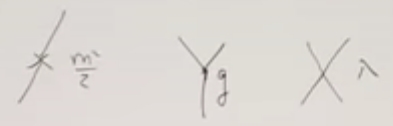
\includegraphics[width=\textwidth]{3-1-feynman-vertices}
		\end{subfigure}
			\begin{subfigure}[t]{0.45\textwidth}
			\caption{Propagator $\braket{0|\Phi(y)\Phi(x)|0}$: amplitude that particle created at $x$ found at $y$. Dimension $[l^-2]$--$\frac{1}{|x-y|^2} if no mass$. If x and y close, propagator blows up--this is the source of all divergences in QFT.}\label{fig:3-1-feynman-propagator}
		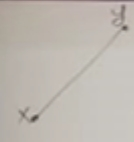
\includegraphics[width=\textwidth]{3-1-feynman-propagator}
	\end{subfigure}
	\end{center}
\end{figure}

\url{https://youtu.be/W6srShxBCrk?t=2227}
	
\section{Fermions and bosons}

TBP

\section{Propagators and renormalization of mass}

TBP

\section{Symmetry and Grassmann numbers}

TBP

\section{A first supersymmetric model}

TBP

\section{Supersymmetry building blocks}

TBP

\section{Lagrangians that preserve supersymmetry}

TBP

\section{Generalizing supersymmetry to 3+1 spacetime, and QFT}

TBP

\section{Supersymmetry breaking and an introduction to grand unified theories}

TBP

\section{GUTs, the SU(5) representation, proton decay}

TBP


\bibliographystyle{unsrt}
\addcontentsline{toc}{section}{Bibliography}
\raggedright
\bibliography{tm}

\end{document}
